\section{Návrh modelových tříd}
V~následujících odstavcích jsou uvedeny všechny modelové třídy, které jsou v~aplikaci obsaženy. Vztahy mezi nimi zobrazuje diagram \ref{fig:model-diagram}.
\begin{figure}[h]
    \centering
    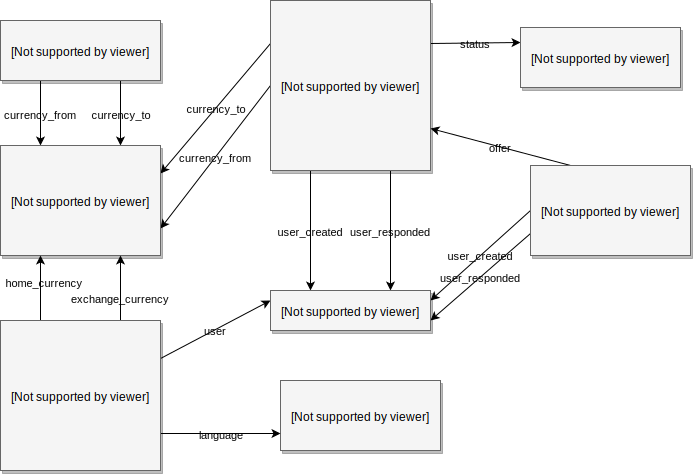
\includegraphics[width=1.0\textwidth]{media/model-diagram}
    \caption{Diagram vztahů modelových tříd}
    \label{fig:model-diagram}
\end{figure}

\paragraph*{Currency} představuje měnu, ze které, respektive do které, lze směnit peníze. Její strukturu lze vidět v~tabulce \ref{tab:model-currency}.
\begin{table}[h]
    \centering
    \caption{Struktura modelové třídy \texttt{Currency}}\label{tab:model-currency}
    \begin{tabulary}{1.0\textwidth}{ L L L }
        \hline
        \textbf{Název} & \textbf{Datový typ} & \textbf{Popis} \\ \hline
         id & int(11) & primární klíč \\
         name & varchar(50) & název \\
         identificator & varchar(3) & třípísmenný identifikátor \\
         prefix & varchar(5) & prefix při zobrazení měny \\
         postfix & varchar(5) & postfix při zobrazení měny \\
    \end{tabulary}
\end{table}

\paragraph*{CurrencyRates} představuje kurz mezi dvěma měnami. Strukturu lze vidět v~tabulce \ref{tab:model-currency-rates}.
\begin{table}[h]
    \centering
    \caption{Struktura modelové třídy \texttt{CurrencyRates}}\label{tab:model-currency-rates}
    \begin{tabulary}{1.0\textwidth}{ L L L }
        \hline
        \textbf{Název} & \textbf{Datový typ} & \textbf{Popis} \\ \hline
         id & int(11) & primární klíč \\
         rate & double & kurz \\
         currency\_from & cizí klíč & měna z~\\
         curency\_to & cizí klíč & měna do \\
    \end{tabulary}
\end{table}

\paragraph*{OfferStatus} představuje stav objednávky. Strukturu lze vidět v~tabulce \ref{tab:model-offer-status}.
\begin{table}[h]
    \centering
    \caption{Struktura modelové třídy \texttt{OfferStatus}}\label{tab:model-offer-status}
    \begin{tabulary}{1.0\textwidth}{ L L L }
        \hline
        \textbf{Název} & \textbf{Datový typ} & \textbf{Popis} \\ \hline
         id & int(11) & primární klíč \\
         title & varchar(50) & název stavu \\
    \end{tabulary}
\end{table}

\paragraph*{Offer} představuje nabídku na směnu peněz. Strukturu lze vidět v~tabulce \ref{tab:model-offer} na straně \pageref{tab:model-offer}.
\begin{table}[h]
    \centering
    \caption{Struktura modelové třídy \texttt{Offer}}\label{tab:model-offer}
    \begin{tabulary}{1.0\textwidth}{ L L L }
        \hline
        \textbf{Název} & \textbf{Datový typ} & \textbf{Popis} \\ \hline
         id & int(11) & primární klíč \\
         lat & double & zeměpisná šířka \\
         lng & double & zeměpisná délka \\
         radius & double & poloměr \\
         amount & int(11) & obnos peněz \\
         exchange\_rate & double & kurz \\
         comment & longtext & komentář k~nabídce \\
         created\_at & datetime & datum vytvoření \\
         updated\_at & datetime & datum poslední aktualizace \\
         currency\_from & cizí klíč & měna z~\\
         currency\_to & cizí klíč & měna do \\
         status & cizí klíč & stav \\
         user\_created & cizí klíč & uživatel, který nabídky vytvořil \\
         user\_responded & cizí klíč & uživatel, který se k~nabídce připojil \\
         address & longtext & adresa \\
    \end{tabulary}
\end{table}

\paragraph*{Feedback} představuje hodnocení uživatele za danou nabídku. Strukturu lze vidět v~tabulce \ref{tab:model-feedback} na straně \pageref{tab:model-feedback}.
\begin{table}[h]
    \centering
    \caption{Struktura modelové třídy \texttt{Feedback}}\label{tab:model-feedback}
    \begin{tabulary}{1.0\textwidth}{ L L L }
        \hline
        \textbf{Název} & \textbf{Datový typ} & \textbf{Popis} \\ \hline
         id & int(11) & primární klíč \\
         comment & longtext & komentář k~hodnocení \\
         stars & int(11) & počet hvězdiček \\
         offer & cizí klíč & nabídka, které se hodnocení týká \\
         user\_created & cizí klíč & uživatel, který přidal hodnocení \\
         user\_responded & cizí klíč & druhý uživatel v~nabídce \\
         created\_at & datetime & datum vytvoření \\
    \end{tabulary}
\end{table}

\pagebreak
\paragraph*{Language} představuje jazyk, do kterého je možné aplikaci přeložit. Strukturu lze vidět v~tabulce \ref{tab:model-language} na straně \pageref{tab:model-language}.
\begin{table}[h]
    \centering
    \caption{Struktura modelové třídy \texttt{Language}}\label{tab:model-language}
    \begin{tabulary}{1.0\textwidth}{ L L L }
        \hline
        \textbf{Název} & \textbf{Datový typ} & \textbf{Popis} \\ \hline
         id & int(11) & primární klíč \\
         identificator & varchar(10) & dvoupísmenný identifikátor \\
         name & varchar(50) & název \\
    \end{tabulary}
\end{table}

\paragraph*{UserProfile} obohacuje třídu výchozího uživatele o~parametry z~tabulky \ref{tab:model-user-profile} na straně \pageref{tab:model-user-profile}.
\begin{table}[h]
    \centering
    \caption{Struktura modelové třídy \texttt{UserProfile}}\label{tab:model-user-profile}
    \begin{tabulary}{1.0\textwidth}{ L L L }
        \hline
        \textbf{Název} & \textbf{Datový typ} & \textbf{Popis} \\ \hline
         id & int(11) & primární klíč \\
         user & cizí klíč & uživatel \\
         profile\_photo & soubor & profilová fotka \\
         address & varchar(255) & adresa \\
         basic\_information & longtext & textová informace o~uživateli \\
         exchange\_currency & cizí klíč & preferovaná domácí měna \\
         home\_currency & cizí klíč & preferovaná druhá měna \\
         radius & double & poloměr \\
         language & cizí klíč & preferovaný jazyk uživatele \\
         lat & double & zeměpisná šířka \\
         lng & double & zeměpisná délka \\
         phone & varchar(20) & telefon \\
    \end{tabulary}
\end{table}